\documentclass[../../main/main.tex]{subfiles}
\graphicspath{{./figures/}}

\setlength{\mtcindent}{-10pt}
\mtcsetoffset{minitoc}{-10pt}

\dominitoc
\faketableofcontents

\makeatletter
\renewcommand{\@chapapp}{\'Electrocin\'etique -- chapitre}
\makeatother

\toggletrue{student}
\HideSolutionstrue
\toggletrue{corrige}
% \renewcommand{\mycol}{black}
\renewcommand{\mycol}{gray}

\begin{document}
\setcounter{chapter}{4}

\chapter{Circuits \'electriques en r\'egime sinuso\"idal forc\'e}

\vfill

\begin{prgm}
	\begin{tcb}*(ror)"know"{Savoirs}
		\begin{itemize}[label=$\diamond$, leftmargin=10pt]
			\item Établir et connaître l'impédance d'une résistance, d'un
			      condensateur, d'une bobine.
			\item Oscillateur électrique ou mécanique soumis à une excitation
			      sinusoïdale.
		\end{itemize}
	\end{tcb}

	\begin{tcb}*(ror)"how"{Savoir-faire}
		\begin{itemize}[label=$\diamond$, leftmargin=10pt]
			\item Remplacer une association série ou parallèle de deux impédances par
			      une impédance équivalente.
			\item Utiliser la représentation complexe pour étudier le régime forcé.
		\end{itemize}
	\end{tcb}
\end{prgm}

\vfill
\minitoc
\vfill

\newpage

Jusque-là en électrocinétique, nous avons étudié la réponse d'un circuit
(c'est-à-dire la tension de sortie) de systèmes linéaires soumis à une
modification rapide de l'entrée (régime libre et échelon montant) d'une valeur
constante à une autre. Nous avons alors observé la présence d'un régime
\textbf{transitoire} suivi d'un régime \textbf{permanent \xul{constant}}.
Dans ce chapitre, nous allons voir la réponse d'un circuit à une entrée
\textbf{sinusoïdale}, qui donnera lieu à un régime transitoire suivi d'un régime
\textbf{permanent \xul{sinusoïdal}}. D'une manière générale, on se
concentre sur la réponse du système une fois le régime permanent établi. On
définit donc

\begin{tcb}[label=def:rsf](defi){Régime sinusoïdal forcé}
	On appelle \textbf{régime sinusoïdal forcé} le régime permanent d'un circuit
	électrique soumis à une entrée sinusoïdale.
	\smallbreak
	Dans tout le chapitre, on supposera donc que l'entrée est allumée depuis une
	durée suffisamment longue pour considérer que le régime transitoire est
	terminé.
	\begin{center}
		\sswitch{
			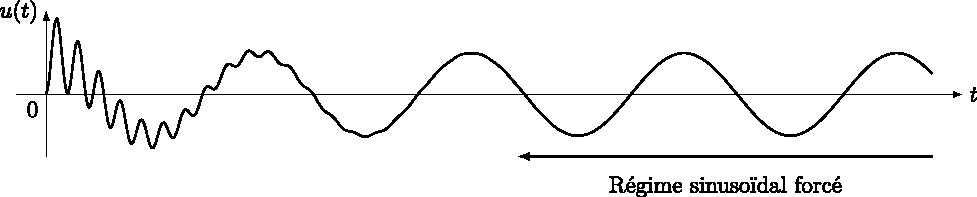
\includegraphics[width=.7\linewidth, draft=true]{rsf_transi}
		}{
			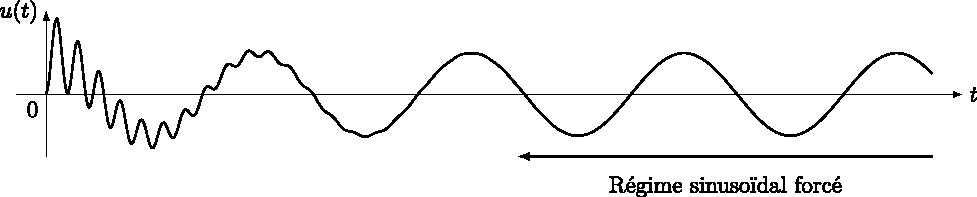
\includegraphics[width=.7\linewidth]{rsf_transi}
		}
		\captionof{figure}{Exemple d'un signal en RSF.}
	\end{center}
\end{tcb}

\section{Circuit RC série en RSF}
\subsection{Présentation}
\noindent
\begin{minipage}[t]{.45\linewidth}
	Soit le circuit RC série, avec $e(t) = E_0\cos(\wt)$.
	\begin{center}
		\sswitch{
			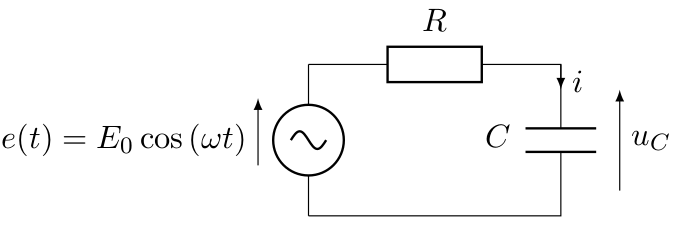
\includegraphics[width=\linewidth, draft=true]{rc_rsf}
		}{
			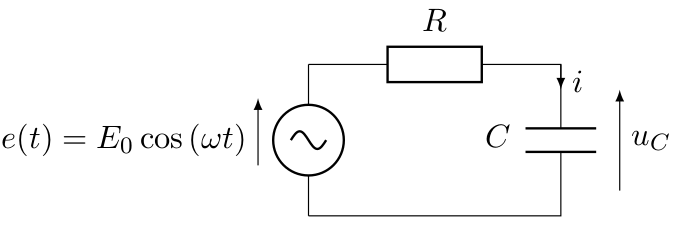
\includegraphics[width=\linewidth]{rc_rsf}
		}
		\captionof{figure}{RC en RSF.}
	\end{center}
\end{minipage}
\hfill
\begin{minipage}[t]{.5\linewidth}
	On applique la LdM~:
	\psw{
		\begin{DispWithArrows*}[fleqn, mathindent=-5pt]
			u_R + u_C &= e(t)
			\Arrow{$u_R = Ri$}
			\\\Lra
			Ri + u_C &= e(t)
			\Arrow{$i = C \dv{u_C}{t}$}
			\\\Lra
			RC \dv{u_C}{t} + u_C &= e(t)
			\Arrow{Forme canonique}
			\\\Lra
			\Aboxed{ \dv{u_C}{t} + \frac{1}{\tau}u_C &= \frac{1}{\tau}E_0\cos(\wt)}
		\end{DispWithArrows*}
		avec $\tau = RC$ la constante de temps.
	}
\end{minipage}
\bigbreak
Résoudre cette équation différentielle demande comme précédemment de trouver la
solution homogène et la solution particulière. La solution homogène est la
solution de
\begin{gather*}
	\dv{u_{C,h}}{t} + \frac{1}{\tau}u_{C,h} = 0
	\Ra
	u_{C,h}(t) = A\exp \left( - \frac{t}{\tau} \right)
\end{gather*}
Pour la solution particulière, \textbf{on admet} qu'elle est de la forme
\begin{gather*}
	\psw{
		u_{C,p}(t) = U\cos(\wt + \f)
	}
\end{gather*}
ce qui donne une solution générale
\psw{
	\[\boxed{u_C(t) = A\exp \left( - \frac{t}{\tau} \right) + U\cos(\wt + \f)}\]
}
\vspace{-15pt}
\begin{tcb}[label=ror:CIounon](impo){Important}
	$K$ dépend des conditions initiales, mais
	\smallbreak \centering\large
	$U$ et $\f$ dépendent du circuit (ici, $R$, $C$, $\w$ et $E_0$).
\end{tcb}

\subsection{Réponse d'un système en RSF}
En supposant le régime permanent établi (définition du RSF), on a donc~:
\begin{tcb}[label=prop:sortiersf](ror){Forme de la réponse d'un système en RSF}
	\psw{
		Pour un signal d'entrée
		\[
			e(t) = E_0 \cos(\wt)
			\quad(\text{ou}\quad
			\eta(t) = \eta_0\cos(\wt))
		\]
		les différentes tensions et intensités dans le circuit oscilleront \textbf{à
			la même pulsation $\w$}, et seront de la forme
		\[
			u(t) = U\cos(\wt+\f_u)
			\qet
			i(t) = I\cos(\wt+\f_i)
		\]
		où $U,I$ et $\f_{u,i}$ sont deux constantes dépendant du système et de
		l'excitation $\w$.
	}
\end{tcb}
\begin{tcb}[cnt, bld](impl)<lfnt>{}
	L'objectif de ce chapitre est de donc de savoir déterminer $U$ et $\f$.
\end{tcb}
\subsection{Passage en complexes}
Une méthode de résolution est d'introduire la formule $U\cos(\wt+\f)$ dans
l'équation différentielle et de rechercher $U$ et $\f$. Si c'est possible, c'est
très calculatoire (cf.\ cours de maths). L'utilisation des nombres complexes
permet de réduire drastiquement cette difficulté.

\begin{tcb}(tool){Méthode}
	Pour cela, on remplace $u(t)$ et $e(t)$ par leurs formes complexes~:
	\psw{
		\begin{gather*}
			\xul{u_C} = \xul{U}\exr^{\jwt}
			\qavec
			\xul{U} = U\exr^{\jj\f}
			\qet
			\xul{e} = E_0\exr^{\jwt}
		\end{gather*}
	}
	Pour revenir aux valeurs réelles après calcul, on prendra donc
	\psw{
		\begin{gather*}
			U_C = \abs{\xul{U_C}}
			\qet
			\f = \arg*{\xul{U_C}}
		\end{gather*}
	}
\end{tcb}

\begin{tcb}(appl){Application}
	Trouver la relation entre l'amplitude complexe $\xul{U_C}$ et les paramètres
	du circuit.
	\tcblower
	\begin{isd}[lefthand ratio=.3]
		\psw{
			À partir de l'équation différentielle, on remplace les valeurs réelles par
			les valeurs complexes, en se rappelant que dériver en complexes revient à
			multiplier par $\jw$~:
		}
		\tcblower
		\psw{
			\begin{DispWithArrows*}[fleqn, mathindent=5pt]
				\tau\dot{\xul{u_C}} + \xul{u_C}    & = \xul{e}
				\Arrow{$\uu_C = \Uu\exr^{\jwt}$}
				\\\Lra
				RC\jw\xul{U}\cancel{\exr^{\jwt}} +
				\xul{U}\cancel{\exr^{\jwt}}                          & =
				E_0\cancel{\exr^{\jwt}}
				\Arrow{On factorise}
				\\\Lra
				\xul{U_C} \left( RC\jw + 1 \right) & = E_0
				\Arrow{On isole}
				\\\Lra
				\Aboxed{
					\xul{U_C}                          & = \frac{E_0}{1 + \jj RC\w}}
			\end{DispWithArrows*}
		}
	\end{isd}
\end{tcb}
Il ne reste plus qu'à prendre le module de $\xul{U_C}$ pour avoir l'amplitude
réelle, et l'argument de $\xul{U_C}$ pour avoir la phase à l'origine des
temps.
\begin{tcb}[sidebyside](rapp)<lftt>{Rappel}
	Pour cela, on rappelle que pour $\xul{z} \in \Cb$ tel que $\xul{z} = x + \jj
		y$, on a
	\[ \abs{\xul{z}} = \sqrt{x^2 + y^2}\]
	% Notamment, le module d'un nombre réel pur est égal à sa valeur absolue,
	% et celui d'un nombre complexe pur à la valeur absolue de sa partie
	% imaginaire.
	\tcblower
	De plus, \textbf{le module d'un rapport est égal au rapport des modules}~:
	$\forall (\xul{z_1}, \xul{z_2}) \in \Cb^2$,
	\[
		\abs{\frac{\xul{z_1}}{\xul{z_2}}} =
		\frac{\abs{\xul{z_1}}}{\abs{\xul{z_2}}}
	\]
\end{tcb}
\begin{tcb}(appl){Application}
	Déterminer donc la valeur réelle de l'amplitude de la solution en RSF.
	\tcblower
	\psw{
		Ainsi,
		\begin{gather*}
			U_C
			= \abs{\xul{U_C}}
			= \abs{\frac{E_0}{1 + \jj RC\w}}
			= \frac{\abs{E_0}}{\abs{1 + \jj RC\w}}
			\\\Lra
			\boxed{
				U_C = \frac{E_0}{\sqrt{1+(RC\w)^2}}
			}
		\end{gather*}
	}
\end{tcb}
On fait de même pour la phase, avec pour rappel~:
\begin{tcb}[sidebyside](rapp)<lftt>{Rappel~: pour $\xul{z} \in \Cb$}
	\[\tan(\arg*{\xul{z}}) = \frac{\Im(\xul{z})}{\Re(\xul{z})}
		\qquad
		\cos(\arg*{\xul{z}}) = \frac{\Re(\xul{z})}{\abs{\xul{z}}}
	\]
	\[
		\qquad
		\sin(\arg*{\xul{z}}) = \frac{\Im(\xul{z})}{\abs{\xul{z}}}
		\qquad
	\]
	On rappelle également que $\tan(-x) = -\tan(x)$.
	\tcblower
	Mais encore,
	\textbf{l'argument d'un rapport est égal à la différence des arguments}~:
	$\forall (\xul{z_1}, \xul{z_2}) \in \Cb^2$,
	\[
		\boxed{
			\arg*{ \frac{\xul{z_1}}{\xul{z_2}} } =
			\arg*{\xul{z_1}} - \arg*{\xul{z_2}}
		}
	\]
\end{tcb}
\begin{tcb}(appl){Application}
	Déterminer la phase à l'origine de la solution du système, sous la forme
	$\tan(\f) = \ldots$ puis $\f = \ldots$. Le passage de l'un à l'autre est-il
	évident~?
	\tcblower
	\psw{
		Ainsi,
		\begin{gather*}
			\f
			= \arg*{ \frac{E_0}{1+\jj RC\w} }
			= \underbrace{\arg*{E_0}}_{=0} - \arg (1+\jj RC\w)
			\\\Ra
			\tan(\f)
			= - \tan(\arg*{1+\jj RC\w})
			= - \frac{RC\w}{1}
		\end{gather*}
		En appliquant $\arctan()$, on obtient
		\[\boxed{\f = -\arctan(RC\w)}\]
	}
\end{tcb}
D'une manière générale, on utilisera l'expression de la tangente d'un
argument \textbf{avant} de voir si on peut prendre l'arctangente de la
tangente.
\begin{tcb}(impo){Attention}
	Ça peut être une réponse acceptable dans certaines conditions, mais bien souvent
	on souhaite exprimer la phase directement. Dans ce cas, il faut faire attention
	au fait que
	\[
	\arctan(\tan(\theta)) = \theta
	\Lra
	\theta \in \left] - \frac{\pi}{2}\,; \frac{\pi}{2} \right[
		\]
		Une manière de s'assurer de l'appartenance de $\theta$ à cet intervalle, il
		suffit de regarder la \textbf{partie réelle} de l'argument, ou bien son
		cosinus~: s'il est positif, alors on a en effet $\theta \in \left] -
	\frac{\pi}{2}\,; \frac{\pi}{2} \right[$. Ici,
		\begin{gather*}
			\cos(\arg*{\f})
			= \frac{\Re(\arg*{\f})}{\abs{\xul{z}}}
			= \frac{1}{\sqrt{1 + (RC\w)^2}} > 0
		\end{gather*}
		donc on peut bien dire que $\arctan\tan(\f) = \f$.
		\smallbreak
		Si ça n'est pas le cas, il faut ajouter ou soustraire $\pi$ à l'argument.
\end{tcb}
% TODO: graphiques pour expliquer si on ajoute ou soustrait \pi.

\begin{tcb}(prop){Résultat}
	La solution particulière est
	\psw{
		\begin{gather*}
			\boxed{u_C (t) = U_C\cos(\wt + \f)}
			\\\text{avec}\\
			\boxed{U_C = \frac{E_0}{\sqrt{1+(RC\w)^2}}}
			\qet
			\boxed{\f = -\arctan(RC\w)}
		\end{gather*}
	}
\end{tcb}

\begin{tcb}(rema)<lfnt>{Remarque~: dépendance en $\w$}
	Comme on l'a vu, le signal de sortie sera à la même pulsation que le signal
	d'entrée, mais par cet exemple du circuit RC on note que la phase et
	l'amplitude \textbf{dépendent de la pulsation}.
\end{tcb}

% \begin{tcb}*(expe)<itc>"trans"{Transition}
% 	À partir de cet exemple, est-ce qu'on peut étendre l'utilisation des
% 	complexes pour le RSF aux lois de bases de l'électrocinétique~?
% \end{tcb}

\section{Circuits électriques en RSF}
Comme au début de l'année, nous nous plaçons toujours dans l'Approximation des
Régimes Quasi-Stationnaires (ARQS), c'est-à-dire que pour un circuit de taille
$L$ alimenté par une source sinusoïdale de fréquence $f$, on doit avoir
\fbox{$Lf \ll c$} avec $c$ la célérité de la lumière/des ondes
électromagnétiques.

\subsection{Lois de l'électrocinétique}
\subsubsection{Loi des nœuds en RSF}
\noindent
\begin{minipage}[t]{.48\linewidth}
	Soit un nœud où se rejoignent 5 branches. Dans l'ARQS, nous avions
	la relation ci-contre. En RSF, les intensités sont sinusoïdales \textbf{et
		de même pulsation} $\w$~: on aurait donc
\end{minipage}
\hfill
\begin{minipage}[t]{.48\linewidth}
	~
	\vspace{-50pt}
	\begin{center}
		\sswitch{
			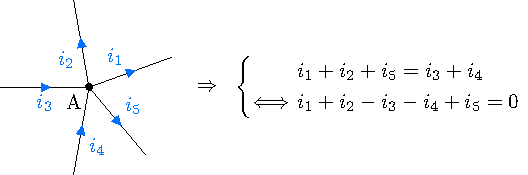
\includegraphics[width=\linewidth, draft=true]{ldn}
		}{
			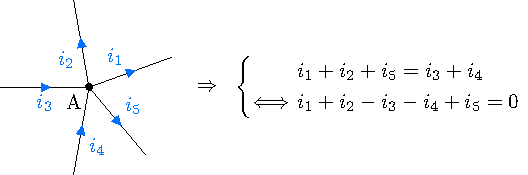
\includegraphics[width=\linewidth]{ldn}
		}
		\captionof{figure}{Loi des nœuds}
	\end{center}
\end{minipage}
\[
	i_1(t) = I_1\cos(\wt+\f_1)
	\qet
	i_2(t) = I_2\cos(\wt+\f_2)
	\qet
	…
\]

\begin{tcb}(prop){Propriété}
	Ainsi, en passant en complexes, on aura
	\psw{
		\begin{gather*}
			\xul{i_1} + \xul{i_2} + \xul{i_5} = \xul{i_3} + \xul{i_4}
			\Lra
			\boxed{\xul{I_1} + \xul{I_2} + \xul{I_5} = \xul{I_3} + \xul{I_4}}\\
			\text{avec}\quad
			\xul{i_k} = I_k\exr^{\jj\f_k}\exr^{\jwt}
			\qet
			\xul{I_k} = I_k\exr^{\jj\f_k}
		\end{gather*}
	}
	\begin{center}
		\textbf{On a donc bien la même relation avec les grandeurs complexes et
			leurs amplitudes complexes}.
	\end{center}
\end{tcb}

\subsubsection{Loi des mailles}
% \begin{wrapfigure}[4]{R}{.5\linewidth}
% 	\vspace*{-30pt}
% 	\centering
% 	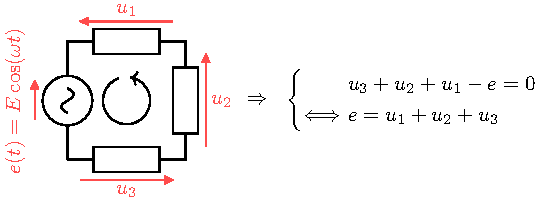
\includegraphics[width=\linewidth]{ldm_rsf}
% \end{wrapfigure}
\noindent
\begin{minipage}[t]{.48\linewidth}
	Soit une maille avec des dipôles quelconques, alimentée par une tension
	sinusoïdale $e(t) = E\cos(\wt)$. Dans l'ARQS, nous avions la relation ci-contre.
	En RSF, les tensions sont sinusoïdales \textbf{et de même pulsation} $\w$~: on
	aurait donc
\end{minipage}
\hfill
\begin{minipage}[t]{.48\linewidth}
	~
	\vspace{-40pt}
	\begin{center}
		\sswitch{
			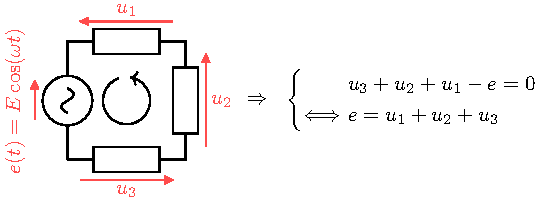
\includegraphics[width=\linewidth, draft=true]{ldm_rsf}
		}{
			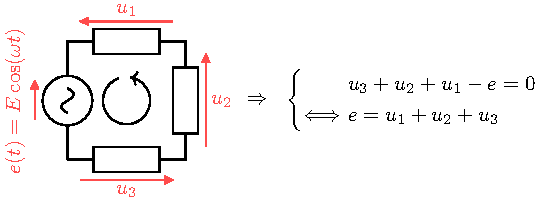
\includegraphics[width=\linewidth]{ldm_rsf}
		}
		\captionof{figure}{Loi des mailles.}
	\end{center}
\end{minipage}
\[
	u_1(t) = U_1\cos(\wt+\f_1)
	\qet
	u_2(t) = U_2\cos(\wt+\f_2)
	\qet
	…
\]

\begin{tcb}(prop){Propriété}
	Ainsi, en passant en complexes, on aura
	\psw{
		\begin{gather*}
			\xul{e} = \xul{u_1} + \xul{u_2} + \xul{u_3}
			\Lra
			\boxed{\xul{E} = \xul{U_1} + \xul{U_2} + \xul{U_3}}\\
			\text{avec}\quad
			\xul{u_k} = U_k\exr^{\jj\f_k}\exr^{\jwt}
			\qet
			\xul{U_k} = U_k\exr^{\jj\f_k}
		\end{gather*}
	}
	\begin{center}
		\textbf{On a donc bien la même relation avec les grandeurs complexes et
			leurs amplitudes complexes}.
	\end{center}
\end{tcb}

\subsection{Impédance et admittance complexes d'un dipôle passif}
\subsubsection{Définition}
En complexes, pour chaque dipôle on aura
\begin{align*}
	\psw{
		u(t) = U\cos(\wt+\f_u)
	}
	 & \qet
	\psw{
		i(t) = I\cos(\wt+\f_i)
	}
	\\
	\beforetext{$\Longrightarrow$}
	\psw{
		\xul{u}(t) = U\exr^{\jj(\wt+\f_u)} = U\exr^{\jj\f_u}\exr^{\jwt} =
		\xul{U}\exr^{\jwt}
	}
	 & \qet
	\psw{
		\xul{i}(t) = I\exr^{\jj(\wt+\f_i)} = I\exr^{\jj\f_i}\exr^{\jwt} =
		\xul{I}\exr^{\jwt}
	}
\end{align*}
Ainsi, on peut aisément exprimer une relation courant-tension pour un dipôle
complexe, sous la forme classique $U = RI$ mais en complexes. On peut
tout à fait calculer $\frac{\xul{u}}{\xul{i}}$ pour avoir une proportionnalité
entre les deux~: on appelle cette constante l'\textbf{impédance}, notée
$\xul{Z}$, et on a donc la \textbf{loi d'Ohm complexe}~:

\begin{tcb}[sidebyside](defi){Définition~: impédance}
	\tcbsubtitle{\fatbox{Loi d'Ohm complexe}}
	\psw{
		\begin{gather*}
			\xul{u}(t) = \xul{Z}\xul{i}(t)
			\Lra
			\boxed{\xul{U} = \xul{Z}\times\xul{I}}\\
			\Rightarrow
			\xul{Z}\quad\text{homogène à une résistance}
		\end{gather*}
	}
	\tcblower
	\begin{center}
		\sswitch{
			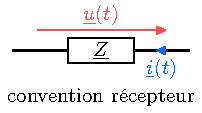
\includegraphics[width=.5\linewidth, draft=true]{zdef}
		}{
			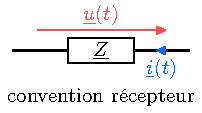
\includegraphics[width=.5\linewidth]{zdef}
		}
		\captionof{figure}{Représentation d'une impédance complexe}
	\end{center}
\end{tcb}

En tant que complexe, on peut prendre son module et son argument~:
\begin{itemize}
	\item Son module $Z = \abs{\xul{Z}}$ est égal au rapport de
	      l'amplitude de $u$ sur celle de $i$~:
	      \psw{
		      \[
			      \boxed{ \abs{\xul{Z}}
				      = \frac{\abs{\xul{u}|}{|\xul{i}}}
				      = \frac{U}{I}
			      }
		      \]
	      }
	\item Son argument $\arg*{\xul{Z}}$ est égal à la différence de phase entre
	      $\xul{u}$ et $\xul{i}$ (aussi appelée \textbf{déphasage}, voir Section
	      ultérieure)~:
	      \psw{
		      \[
			      \boxed{\arg*{\xul{Z}}
				      = \arg*{ \frac{\xul{u}}{\xul{i}} }
				      = \f_u - \f_i}
		      \]
	      }
\end{itemize}

\begin{tcb}(defi){Définition~: admittance}
	Assez naturellement, comme on avait la conductance égale à l'inverse d'une
	résistance, on peut définir l'inverse d'une impédance~: c'est
	l'\textbf{admittance complexe} $\xul{Y}$~:
	\psw{
		\[
			\boxed{\xul{Y}
				= \frac{1}{\xul{Z}} \Rightarrow \xul{I}
				= \xul{Y}\times\xul{U}}
		\]
	}
\end{tcb}

\subsubsection{Impédances de bases}

Pour trouver les impédances des dipôles de base, on utilise leurs relations
courant-tension qu'on convertit en complexes, \textbf{en se souvenant de dériver
	en complexes équivaut à multiplier par $\jw$}.

\begin{tcb}*[tabularx={l|Y|Y|Y}](defi)"ror"
	{Définition~: impédances des dipôles de base}
	&
	\textbf{Résistance} &
	\textbf{Inductance} &
	\textbf{Capacité}
	\\\hline
	\rotatebox[origin=c]{90}{Schéma} &
	\sswitch{
		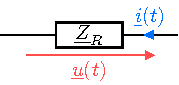
\includegraphics[height=2cm, draft=true]{zr}
	}{
		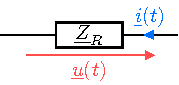
\includegraphics[height=2cm]{zr}
	}
	\captionof{figure}{$\xul{Z_R}$}
	&
	\sswitch{
		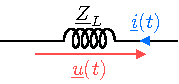
\includegraphics[height=2cm, draft=true]{zl}
	}{
		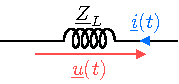
\includegraphics[height=2cm]{zl}
	}
	\captionof{figure}{$\xul{Z_L}$}
	&
	\sswitch{
		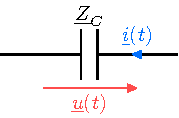
\includegraphics[height=2cm, draft=true]{zc}
	}{
		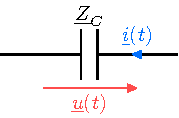
\includegraphics[height=2cm]{zc}
	}
	\captionof{figure}{$\xul{Z_C}$}
	\\\hline
	\rotatebox[origin=c]{90}{Démonstration} &
	\psw{
		$\begin{aligned}
				u(t)              & = Ri(t)       \\
				\Lra
				\xul{u}(t)        & = R\xul{i}(t) \\
				\Lra
				\Aboxed{\xul{Z}_R & = R}
			\end{aligned}$
	}
	&
	\psw{
		$\begin{aligned}
				u(t)              & = L\dv{i}{t}        \\
				\Lra
				\xul{u}(t)        & = \jj L\w\xul{i}(t) \\
				\Lra
				\Aboxed{\xul{Z}_L & = \jj L\w}
			\end{aligned}$
	}
	&
	\psw{
		$\begin{aligned}
				i(t)              & = C\dv{u}{t}         \\
				\Lra
				\xul{i}(t)        & = C\jwt\xul{u}(t)    \\
				\Lra
				\Aboxed{\xul{Z}_C & = \frac{1}{\jj C\w}}
			\end{aligned}$
	}
	\\\hline
\end{tcb}

\subsubsection{Comportements limites}
Ainsi, la résistance ne change pas d'expression entre les réels et les
complexes, alors que les bobines et condensateurs ont des caractéristiques
complexes différentes. En plus de ça, leurs impédances \textbf{dépendent} de
$\w$~: on peut notamment étudier deux cas limites, quand $\w\rightarrow0$ et
$\w\rightarrow+\infty$~:
\begin{tcb}[tabularx*={\renewcommand{\arraystretch}{1.5}}{l|Y|Y}](prop){Propriété}
	&
	$\w\rightarrow0$ &
	$\w\rightarrow+\infty$
	\\\hline
	\rotatebox[origin=c]{90}{Bobine} &
	\psw{
		$\abs{\xul{Z}_L} = L\w \underset{\w\rightarrow0}{\rightarrow}0$
	}
	\smallbreak
	\sswitch{
		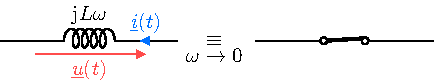
\includegraphics[width=\linewidth, draft=true]{zlwa}
	}{
		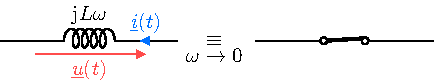
\includegraphics[width=\linewidth]{zlwa}
	}
	\vspace{-15pt}
	&
	\psw{
		$\abs{\xul{Z}_L} = L\w \underset{\w\rightarrow+\infty}{\rightarrow}+\infty$
	}
	\smallbreak
	\sswitch{
		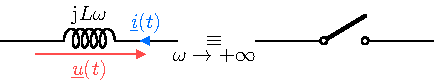
\includegraphics[width=\linewidth, draft=true]{zlwi}
	}{
		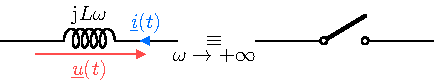
\includegraphics[width=\linewidth]{zlwi}
	}
	\vspace{-15pt}
	\\\hline
	\rotatebox[origin=c]{90}{Condensateur} &
	\psw{
		$\abs{\xul{Z}_C} = 1/(C\w) \underset{\w\rightarrow0}{\rightarrow}+\infty$
	}
	\smallbreak
	\sswitch{
		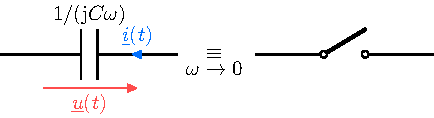
\includegraphics[width=\linewidth, draft=true]{zcwa}
	}{
		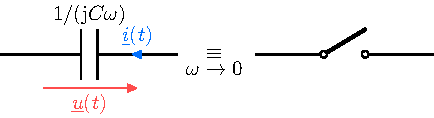
\includegraphics[width=\linewidth]{zcwa}
	}
	\vspace{-15pt}
	&
	\psw{
		$\abs{\xul{Z}_C} = 1/(C\w) \underset{\w\rightarrow+\infty}{\rightarrow}0$
	}
	\smallbreak
	\sswitch{
		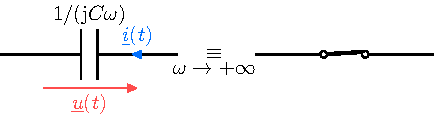
\includegraphics[width=\linewidth, draft=true]{zcwi}
	}{
		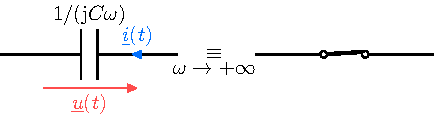
\includegraphics[width=\linewidth]{zcwi}
	}
	\vspace{-15pt}
\end{tcb}
% En effet, l'impédance étant homogène à une résistance, on peut rendre équivalent
% le fait d'avoir une impédance infinie et d'avoir une «~résistance~» infinie,
% c'est-à-dire un interrupteur ouvert, qui ne laisse pas passer le courant. À
% l'inverse, une résistance nulle laisse passer le courant sans résistance, comme
% un fil.

% \vspace{-15pt}
\subsection{Associations d'impédances et ponts diviseurs}
Enfin, comme la relation courant-tension avec l'impédance complexe est analogue
à celle d'une résistance, on peut facilement démontrer que les associations
d'impédances suivent les associations de résistances, et qu'on peut donc
appliquer les ponts diviseurs de tension et de courant comme si on n'avait que
des résistances.
% \vspace{-15pt}
\begin{tcb}[tabularx={l|Y|Y}](ror){Associations d'impédances}
	& \textbf{Schéma} & \textbf{Relations}
	\\\hline
	\rotatebox[origin=c]{90}{\textbf{En série}} &
	\sswitch{
		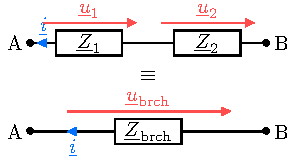
\includegraphics[width=\linewidth, draft=true]{zserie}
	}{
		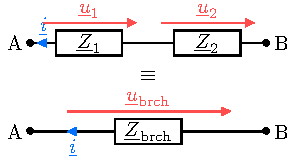
\includegraphics[width=\linewidth]{zserie}
	}
	\vspace{-15pt}
	&
	\begin{itemize}
		\bitem{Impédance équivalente} :
		\psw{
			\[\xul{Z}\ind{eq} = \xul{Z}_1 + \xul{Z}_2\]
		}
		\vspace{-15pt}
		\bitem{Diviseur de tension} :
		\psw{
			\[\xul{u_k} = \frac{\xul{Z}_k}{\xul{Z}_{\rm branche}}\xul{u}\]
		}
		\vspace{-15pt}
	\end{itemize}
	\\\hline
	\rotatebox[origin=c]{90}{\textbf{En parallèle}} &
	\sswitch{
		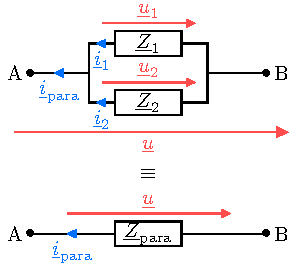
\includegraphics[width=.7\linewidth, draft=true]{zpara}
	}{
		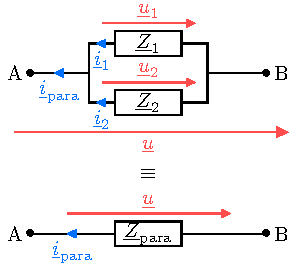
\includegraphics[width=.7\linewidth]{zpara}
	}
	\vspace{-15pt}
	&
	\begin{itemize}
		\bitem{Dipôle équivalent} :
		\psw{
			\begin{gather*}
				\xul{Y}\ind{eq} = \xul{Y}_1 + \xul{Y}_2
				\\\Lra
				\frac{1}{\xul{Z}\ind{eq}} = \frac{1}{\xul{Z}_1} + \frac{1}{\xul{Z}_2}
				\Lra
				\xul{Z}\ind{eq} = \frac{\xul{Z}_1\xul{Z}_2}{\xul{Z}_1+\xul{Z}_2}
			\end{gather*}
		}
		\vspace{-15pt}
		\bitem{Diviseur de courant} :
		\psw{
			\begin{gather*}
				\xul{i_k} = \frac{\xul{Y}_k}{\xul{Y}_{\rm para}}\xul{i}
				\Lra
				\xul{i_k} = \frac{\xul{Z}_{\rm para}}{\xul{Z}_k}\xul{i}\\
				% \Lra
				% \xul{i_{\fbox{1}}} = \frac{\xul{Z}_{\fbox{2}}}{\xul{Z}_1 + \xul{Z}_2}\xul{i}
			\end{gather*}
		}
		\vspace{-30pt}
	\end{itemize}
\end{tcb}

\subsection{Exercices bilan}
\begin{tcb}[sidebyside, righthand ratio=.7](appl){Association d'impédances}
	Quelle est l'impédance de l'association suivante~?
	\begin{center}
		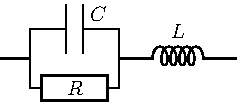
\includegraphics[width=\linewidth]{exo_zeq}
	\end{center}
	\tcblower
	\psw{
		L'association en parallèle donne
		$\frac{\xul{Z}_C\xul{Z}_R}{\xul{Z}_C+\xul{Z}_R}$, et on ajoute $\xul{Z}_L$ à
		celle-ci~:
		\begin{gather*}
			\xul{Z}\ind{eq}
			= \frac{\dfrac{1}{\jj C\w}\times R}{\dfrac{1}{\jj C\w} + R}
			+ \jj L\w
			\Lra
			\boxed{
				\xul{Z}\ind{eq} = \frac{R}{1+\jj RC\w} + \jj L\w}
		\end{gather*}
	}
	\vspace{-15pt}
\end{tcb}

\begin{tcb}[valign=top](appl){Détermination de constantes}
	\begin{isd}[sidebyside align=center]
		Soit le circuit suivant, avec une entrée sinusoïdale $e(t) = E\cos(\wt)$.
		Exprimer l'amplitude complexe $\xul{U}_C$ associée à la tension $u_C$ en
		fonction de $R$, $L$, $C$ et $\w$.
		\tcblower
		\begin{center}
			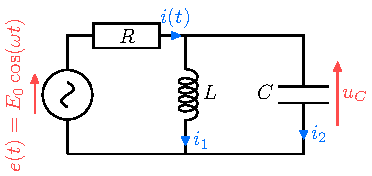
\includegraphics[width=\linewidth]{rlc_r-s-LC-parr}
		\end{center}
	\end{isd}
	\tcblower
	\psw{
		S'il n'y avait pas l'inductance, on pourrait facilement utiliser un pont
		diviseur de tension pour exprimer $\xul{u}_C$ en fonction de $\xul{e}$,
		$\xul{Z}_R$ et $\xul{Z}_C$. Pour se ramener à la situation du pont diviseur de
		tension, on détermine donc une première impédance équivalente issue de
		l'association en parallèle de $L$ et $C$, après les avoir converties en
		complexes~:
		\begin{center}
			\sswitch{
				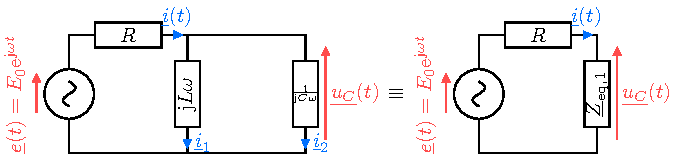
\includegraphics[width=\linewidth, draft=true]{rlc_r-s-LC-parr_cplx}
			}{
				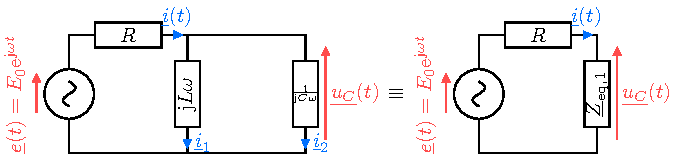
\includegraphics[width=\linewidth]{rlc_r-s-LC-parr_cplx}
			}
		\end{center}
		On peut déterminer $\xul{Z}_{\equ, 1}$ avec les admittances $\xul{Y}_L = 1/\jj
			L \w$ et $\xul{Y}_C = \jj C\w$, et utiliser le pont diviseur de tension
		directement avec l'amplitude complexe~: $\xul{U}_C =
			\frac{\xul{Z}_{\equ,1}}{\xul{Z}_{\equ,1}+\xul{Z}_R}E_0$. Ainsi,
		\begin{gather*}
			\xul{U}_C = \frac{\dfrac{1}{
					\psw[orange]{\cancel{\dfrac{1}{\jj L\w} + \jj C\w}}}}
			{\dfrac{1}{\psw[orange]{\cancel{\dfrac{1}{\jj L\w} + \jj C\w}}}
				+ R\psw[orange]{(…)}}E_0
			\times \psw[orange]{
				\frac{\jj C\w + \dfrac{1}{\jj L\w}}{\jj C\w + \dfrac{1}{\jj L\w}}}
			\Lra
			\xul{U}_C = \frac{1}{1 + \jj RC\w + \dfrac{R}{\jj L\w}}E_0\\
			\Lra
			\boxed{
				\xul{U}_C = \frac{E_0}{1 + \jj \left( RC\w - \dfrac{R}{L\w} \right)}
			}
		\end{gather*}
		où on a simplifié la fraction en multipliant par le terme orange d'abord,
		puis en utilisant que $1/\jj = -\jj$.
	}
\end{tcb}

\subsection{Résumé}

\begin{tcb}(ror){Résumé méthode}
	Un système soumis à une excitation sinusoïdale du type $e(t) = E_0\cos(\wt)$
	se comporte de la manière suivante~:
	\begin{itemize}
		\item On observe un court régime transitoire dû à la solution homogène de
		      l'ED ($A\exr^{-t/\tau}$ pour ordre 1, pseudo-périodique ou apériodique
		      pour l'ordre 2)~;
		\item Après ce régime, on obtient la solution particulière~:
		      \[
			      x(t) = X\cos(\wt+\f_X)
		      \]
		      avec $\w$ la \textbf{pulsation d'entrée}, $X$ et $\f_X$  définies
		      \textbf{par le système} (et non pas des conditions initiales).
		\item Pour trouver ces valeurs, on définit~:
		      \begin{itemize}
			      \item \leftcenters{l'entrée complexe~:}
			            {\psw{$\xul{e}(t) = E_0\exr^{\jwt}$}}
			            \vspace{-10pt}
			      \item \leftcenters{les signaux de sortie complexes~:}
			            {\psw{$\xul{x}(t) = X\exr^{\jj(\wt+\f_X)}$~;}}
			            \vspace{-10pt}
			      \item \leftcenters{les amplitudes complexes~:}
			            {\psw{$\xul{X} = X\exr^{\jj\f_X}
						            \Ra
						            \xul{x}(t) = \xul{X}\exr^{\jwt}$~;}}
			            \vspace{-5pt}
			      \item On retrouve les grandeurs réelles en en prenant le module et
			            la phase~:
			            \psw{
				            \[
					            \boxed{X = \abs{\xul{X}}}
					            \qet
					            \boxed{\f_X = \arg*{\xul{X}}}
				            \]
			            }
			            \vspace{-15pt}
		      \end{itemize}
	\end{itemize}
\end{tcb}

\section{Mesure de déphasages}
\subsection{Définition}
\begin{tcb}(defi){Définition~: déphasage}
	Pour deux signaux sinusoïdaux \textbf{de mêmes fréquences} $s_1(t) =
		S_1\cos(\wt+\f_1)$ et $s_2(t) = S_2\cos(\wt+\f_2)$, on définit le
	\textbf{déphasage} entre $s_2$ et $s_1$ comme étant la \textbf{différence de
		leurs phases instantanées}~:
	\psw{
		\[
			\D\f_{2/1} = (\wt + \f_2) - (\wt+\f_1)
			\Lra
			\boxed{\D\f_{2/1} = \f_2 - \f_1}
		\]
	}
	\vspace{-15pt}
\end{tcb}
% \begin{tcb}(rapp){}
% 	Étant donné que les sorties en RSF ont la même pulsation que l'entrée, on ne
% 	s'intéressera qu'à des signaux de même pulsation/fréquence.
% \end{tcb}

\subsection{Lecture d'un déphasage}

\noindent
\begin{minipage}{0.65\linewidth}
	Le déphasage $\D\f_{2/1} = \f_2 - \f_1$ est lié au \textbf{retard temporel}
	$\D{t}_{2/1} = t_2 - t_1$ du signal $s_2$ par rapport au signal $s_1$~: on a
	\psw{
		\[\boxed{\D\f_{2/1} = -\w\D{t}_{2/1}}\]
	}
	Dans ce cas, le déphasage obtenu est entre $-\pi$ et $+\pi$. On définit~:
	\begin{itemize}
		\item \psw{
			      $\D\f_{2/1} > 0 \Rightarrow s_2$ est en avance sur $s_1$~;
		      }
		\item \psw{
			      $\D\f_{2/1} < 0 \Rightarrow s_2$ est en retard sur $s_1$.
		      }
	\end{itemize}
\end{minipage}
\hfill
\begin{minipage}{0.30\linewidth}
	\vspace{-15pt}
	\begin{center}
		\sswitch{
			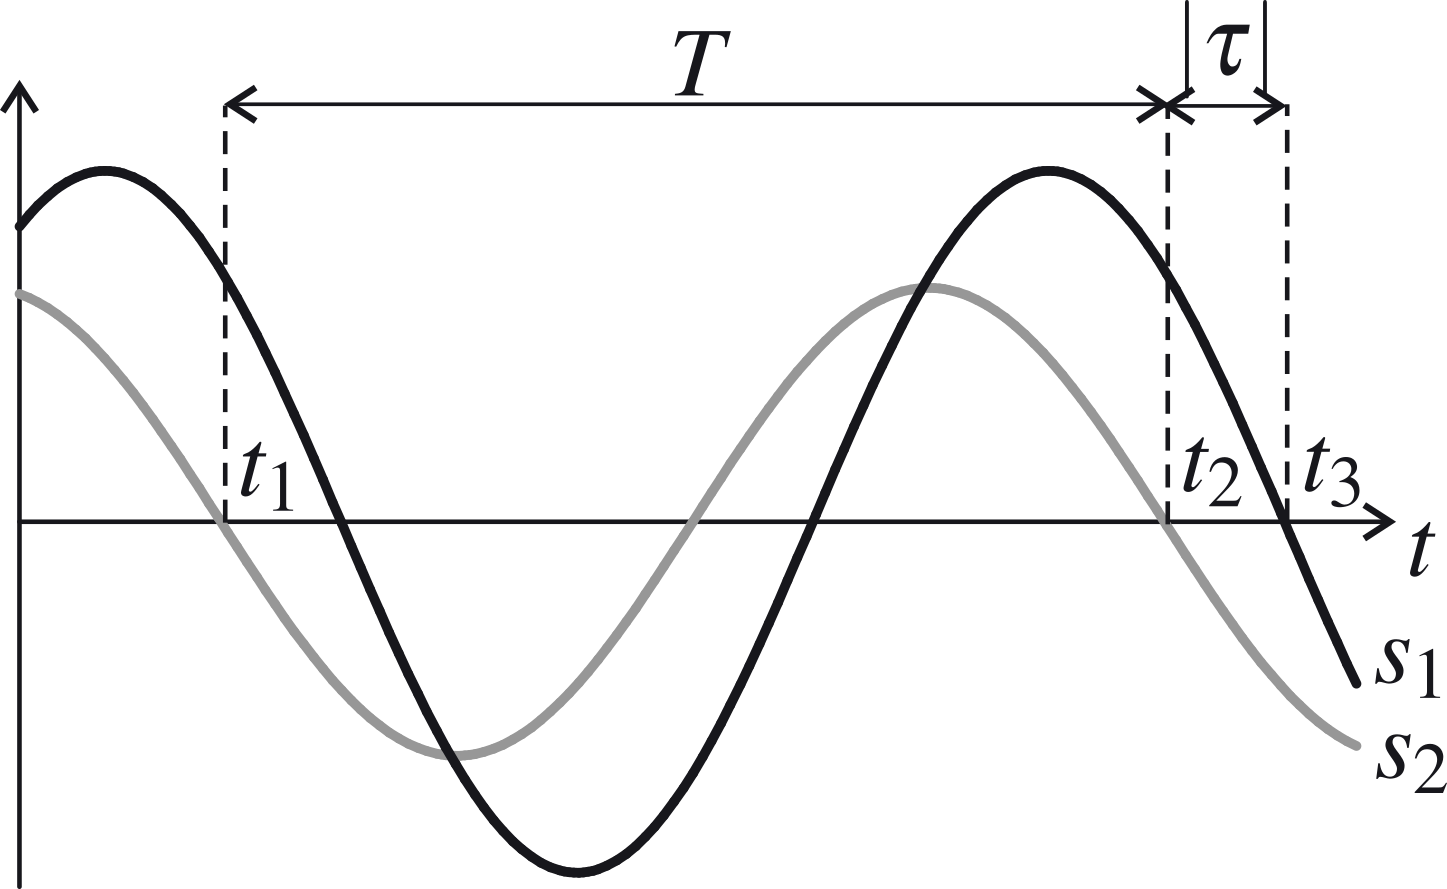
\includegraphics[width=\linewidth, draft=true]{dfretard}
		}{
			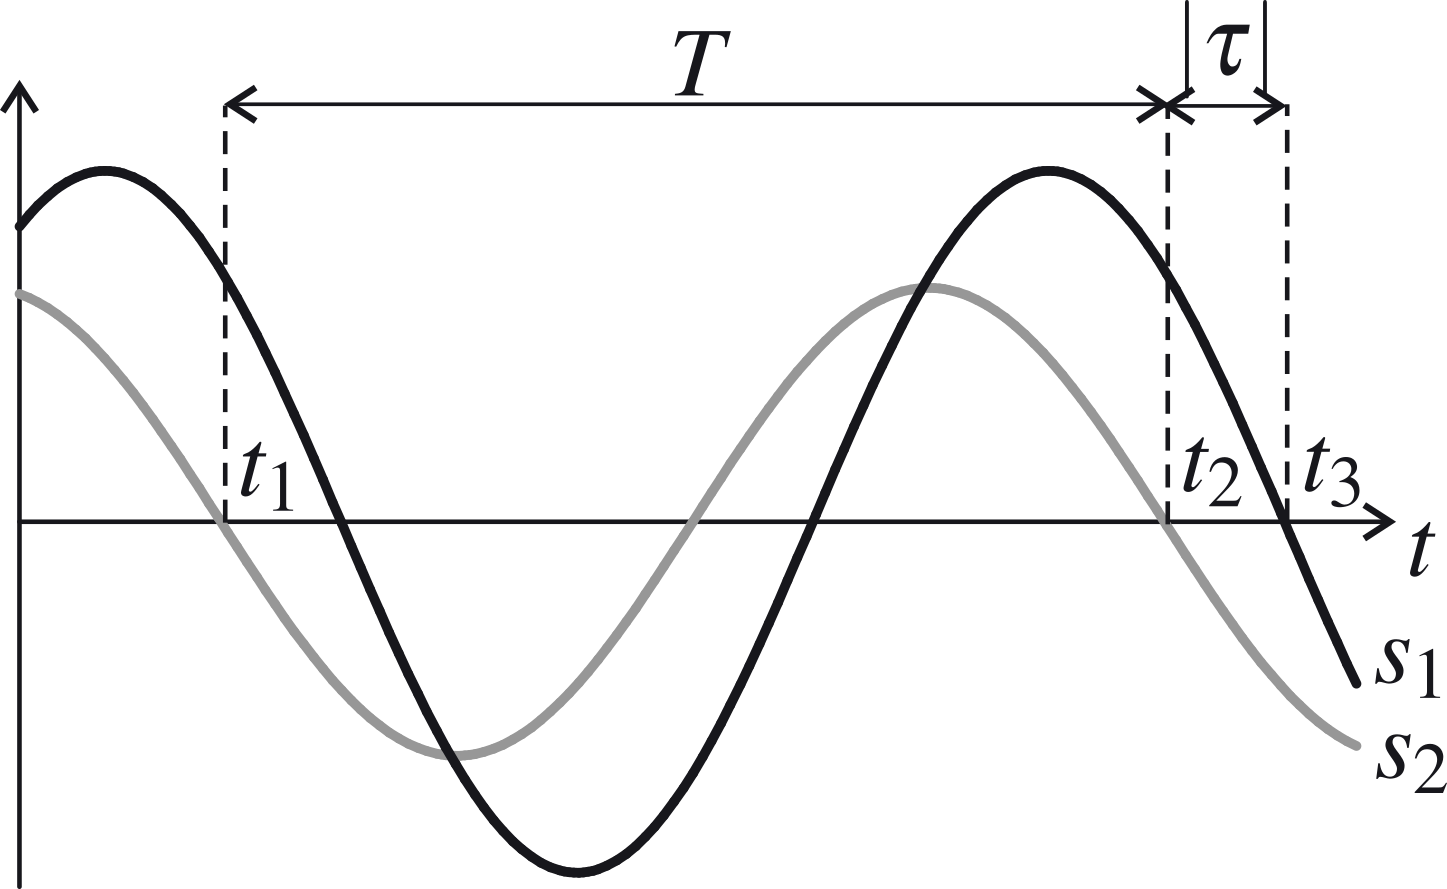
\includegraphics[width=\linewidth]{dfretard}
		}
		\captionof{figure}{Déphasage}
	\end{center}
\end{minipage}

Le principe est de mesurer la différence de temps entre les deux moments les
plus proches tels que les deux signaux s'annulent \textbf{avec la même pente}.
% Par construction, la pulsation représente une vitesse angulaire, c'est pourquoi
% on a $\w = 2\pi/T$ comme $v = d/t$ en mécanique. On trouve donc naturellement la
% relation entre $\D\f_{2/1}$ et $\D{t}_{2/1}$.

\subsection{Valeurs particulières}
\begin{tcb}[sidebyside, righthand ratio=.3](defi){Signaux en phase}
	Deux signaux sont \textbf{en phase} si leur \textbf{déphasage est nul}
	(modulo $2\pi$)~:
	\psw{
		\[
			\D\f \equiv 0\quad[2\pi]
			\Lra
			\boxed{\D\f = 2p\pi} \quad p \in \Zb
		\]
	}
	Les signaux passent par leurs valeurs maximales et minimales aux mêmes
	instants, et s'annulent simultanément.
	\tcblower
	\begin{center}
		\sswitch{
			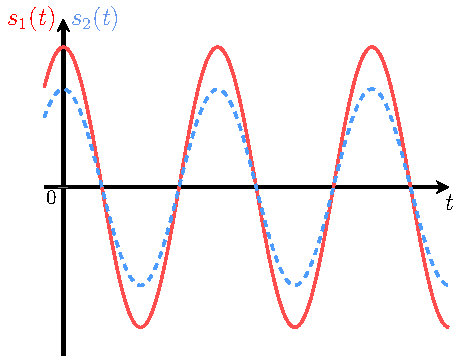
\includegraphics[width=\linewidth, draft=true]{dfeq0.pdf}
		}{
			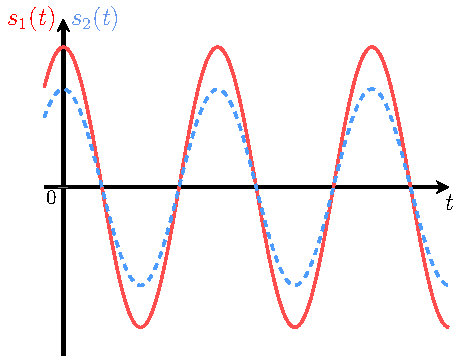
\includegraphics[width=\linewidth]{dfeq0.pdf}
		}
		\vspace{-15pt}
		\captionof{figure}{En phase.}
	\end{center}
\end{tcb}

\begin{tcb}[sidebyside, righthand ratio=.3](defi){Signaux en quadrature de phase}
	Deux signaux sont en \textbf{quadrature phase} si leur déphasage est de
	$\mathbf{\pm\pi/2}$ (modulo $2\pi$)~:
	\psw{
		\[
			\D\f \equiv \pm\frac{\pi}{2} \quad[2\pi]
			\Lra
			\boxed{\D\f = \left( p+\frac{1}{2} \right)\pi}
		\]
	}
	Quand un signal s'annule, l'autre est à son maximum où à son minimum~:
	c'est la relation entre un cosinus et un sinus.
	\tcblower
	\begin{center}
		\sswitch{
			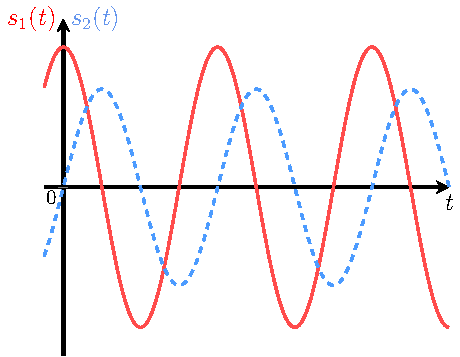
\includegraphics[width=\linewidth, draft=true]{dfeqpi2.pdf}
		}{
			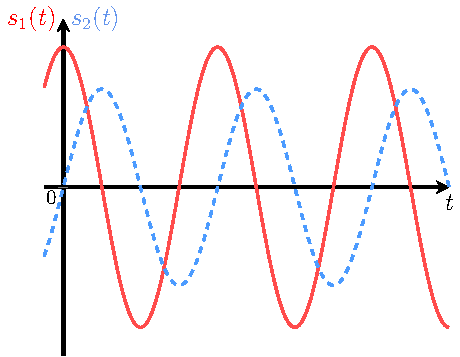
\includegraphics[width=\linewidth]{dfeqpi2.pdf}
		}
		\vspace{-15pt}
		\captionof{figure}{En quadrature.}
	\end{center}
\end{tcb}

\begin{tcb}[sidebyside, righthand ratio=.3](defi){Signaux en opposition de phase}
	Deux signaux sont en \textbf{opposition de phase} si leur déphasage est de
	$\mathbf{\pm\pi}$ (modulo $2\pi$)~:
	\psw{
		\[
			\D\f \equiv \pm\pi \quad[2\pi]
			\Lra
			\boxed{\D\f = (2p+1)\pi}
		\]
	}
	Lorsqu'un signal passe par sa valeur maximale, l'autre est à la valeur
	minimale, mais ils s'annulent simultanément.
	\tcblower
	\begin{center}
		\sswitch{
			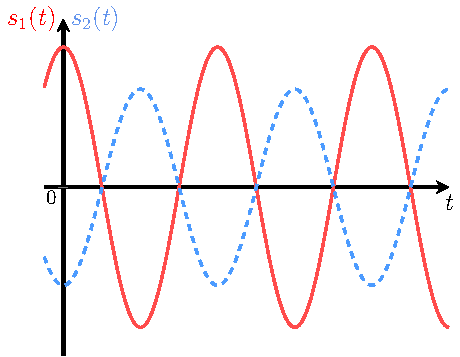
\includegraphics[width=\linewidth, draft=true]{dfeqpi.pdf}
		}{
			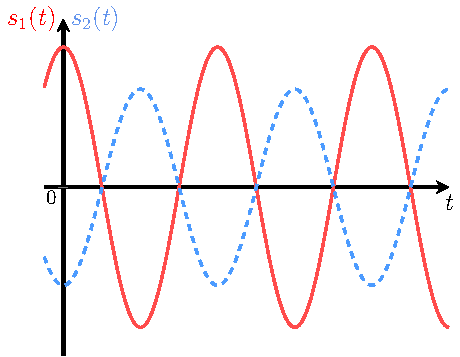
\includegraphics[width=\linewidth]{dfeqpi.pdf}
		}
		\vspace{-15pt}
		\captionof{figure}{En opposition.}
	\end{center}
\end{tcb}

\subsection{Déphasage des impédances}
Pour un dipôle de tension $\xul{U}$ traversé par une intensité $\xul{I}$, on
définit $\xul{Z} = \frac{\xul{U}}{\xul{I}}$, et on a donc $\arg*{\xul{Z}} =
	\arg*{\xul{U}} - \arg*{\xul{I}}$. Ainsi, la phase d'une impédance représente le
déphasage entre la tension et le courant. Pour les différents dipôles
classiques, on trouve~:
\begin{itemize}
	\item \psw{
		      $\arg*{\xul{Z}_R} = 0 \Rightarrow$ signaux en phase~;
	      }
	\item \psw{
		      $\arg*{\xul{Z}_L} = \arg*{\jj L\w} = \pi/2 \Rightarrow$ signaux en
		      quadrature de phase, avec $\xul{u}$ en avance sur $\xul{i}$~;
	      }
	\item \psw{
		      $\arg*{\xul{Z}_C} = \arg*{1/\jj C\w} = -\pi/2 \Rightarrow$ signaux en
		      quadrature de phase, avec $\xul{u}$ en retard sur $\xul{i}$.
	      }
	      \vspace{-15pt}
\end{itemize}

\end{document}
